\section{Koordinatensysteme und Koordinatentransformationen} \label{sec:ks}

Um ein Modellauto steuern zu können, werden unter anderem die Informationen über den aktuellen Standort und den Zielpunkt, den das Fahrzeug ansteuern soll, benötigt. Die Trajektorie ist wiederum davon abhängig, an welcher Stelle sich die Fahrbahnmarkierungen befinden. Alle Positionen von Objekten im Raum werden deshalb mit Entfernungen relativ zu entsprechenden \gls{acr:ks} beschrieben. Für die Beschreibung unseres \gls{glos:tucar} auf dem Parcours und die Lage der Straßenlinien eignet sich das kartesische \gls{acr:ks} besser als Polar- oder Kugelkoordinaten. Es wurden vier hierarchisch angeordnete \gls{acr:ks} festgelegt, welche in Abbildung~\ref{fig:grundlagen_kos} verdeutlicht werden. Letztendlich waren aber nur drei davon in Benutzung. 

\begin{figure}[H] % [htb]
  \centering
  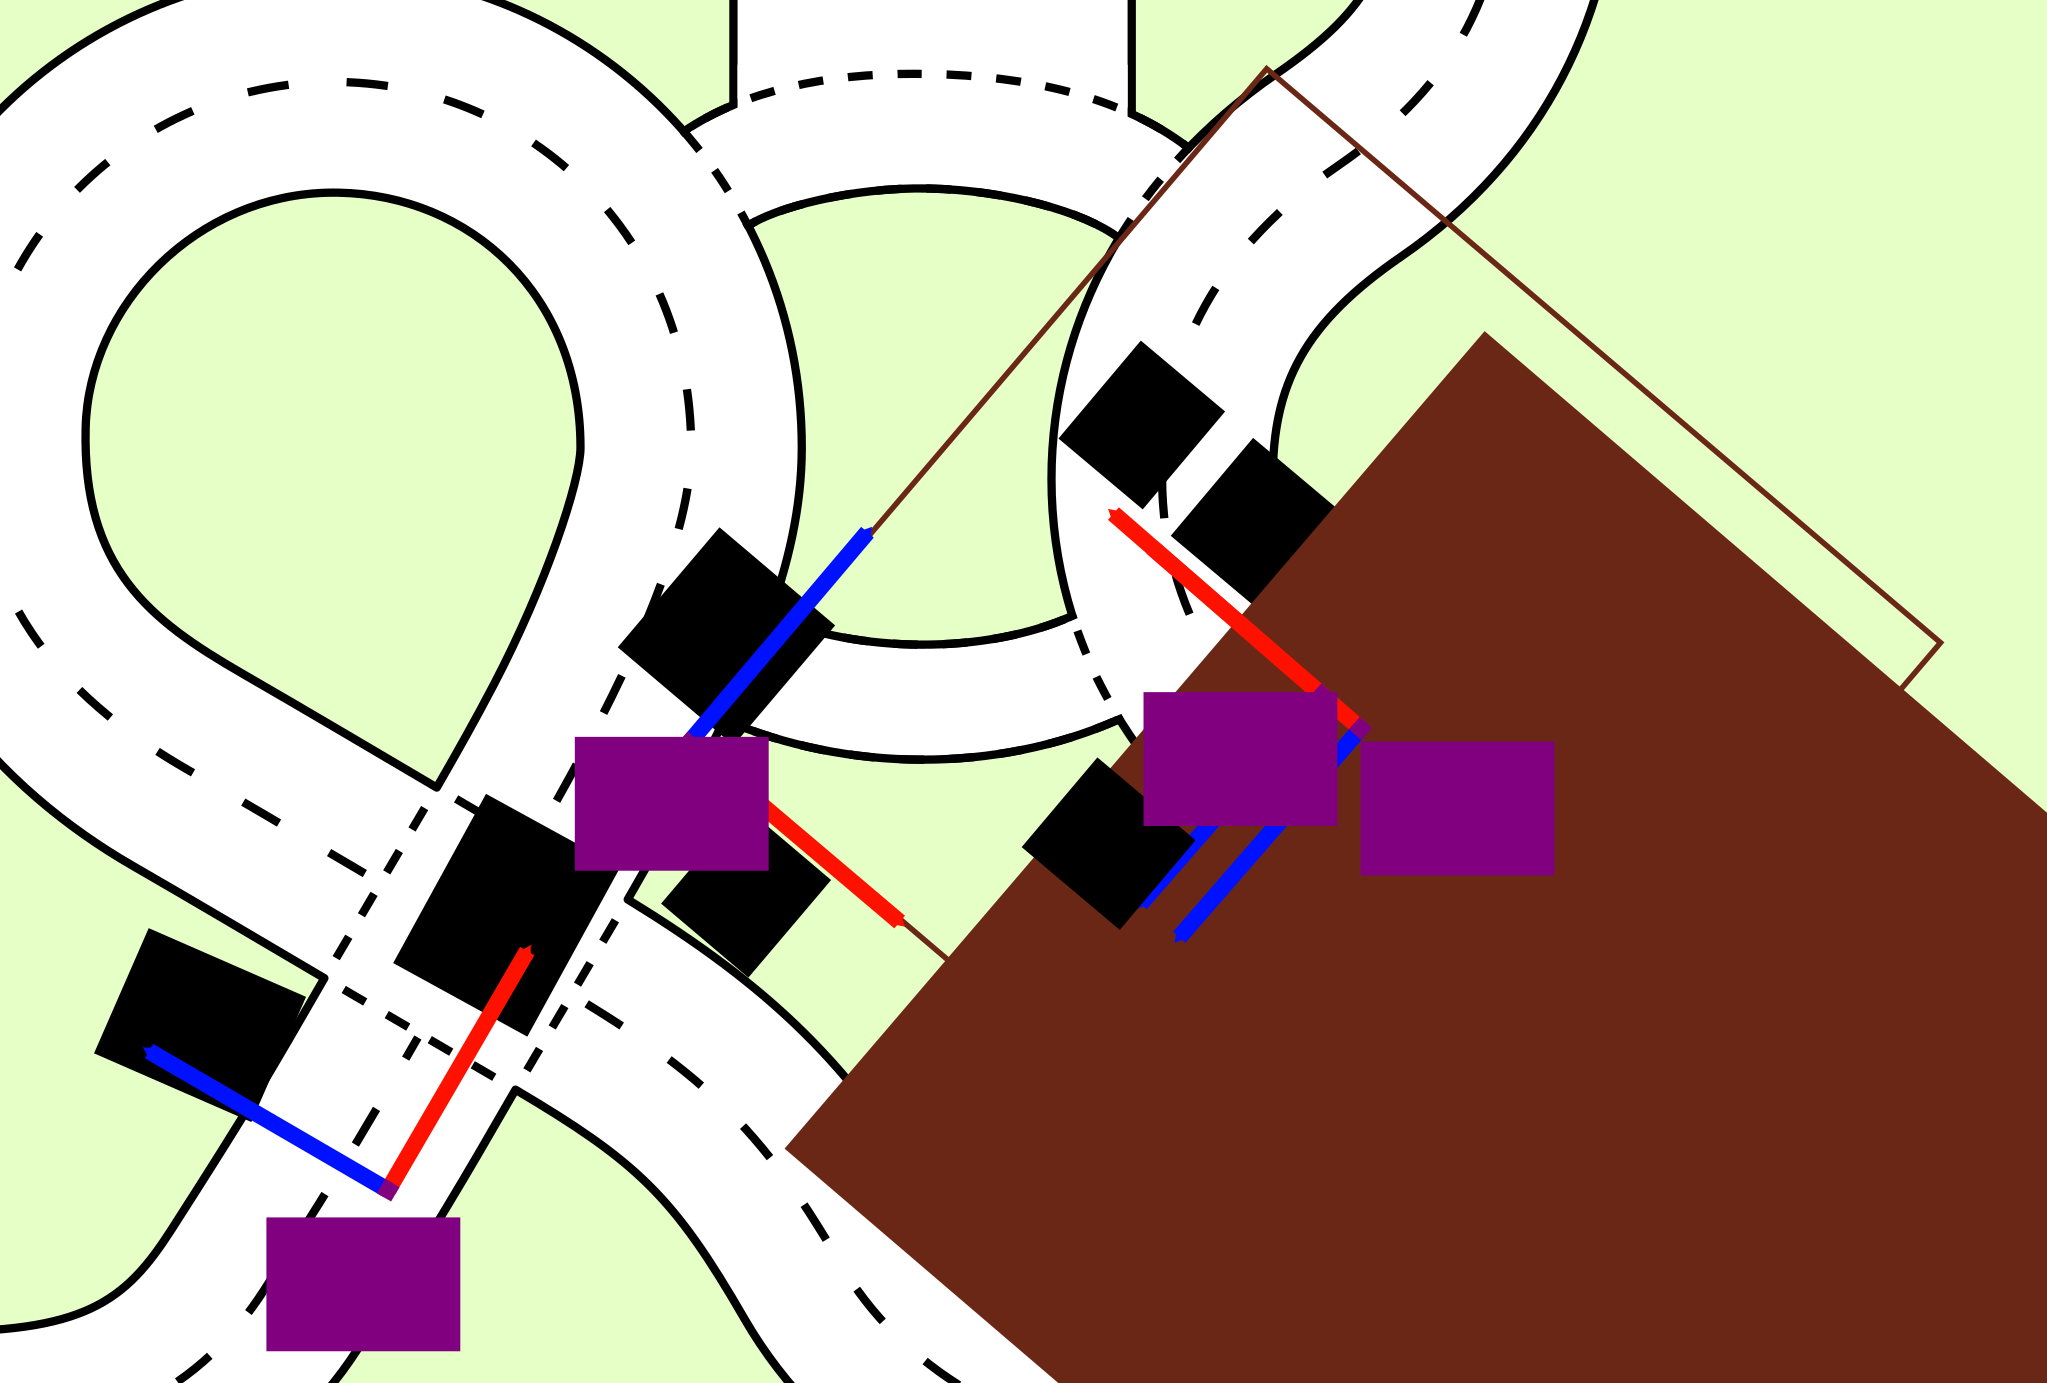
\includegraphics[width=0.9\textwidth]{grundlagen_kos.pdf}
  \caption{Alle eingeführten Koordinatensysteme im Überblick}
  \label{fig:grundlagen_kos}
\end{figure}

Das Weltkoordinatensystem \gls{lat:WeltKOS} bildet die Basis und ist an einem beliebigen Punkt des Szenarios festgemacht. Es dient zur Beschreibung der Pose des mobilen Roboters und der Linienpunkte in der Weltkarte. Damit sich die Pixelkoordinaten des Bildes nicht von der Matrixindizierung unterscheiden, wird das Bildkoordinatensystem \gls{lat:BildKOS} in die linke obere Ecke des entzerrten Fotos gelegt. So zeigt die x-Achse in Richtung der Zeilen und die Spalten laufen mit der y-Koordinate. In der Hinterachse des Autos liegt das Roboterkoordinatensystem \gls{lat:RoboterKOS}, welches in der Lage zum Weltkoordinatensystem die Pose darstellt. Zwischenzeitlich hatten wir zusätzlich ein Linienkoordinatensystem \gls{lat:LinienKOS} festgelegt, welches so in der Bildecke platziert war, dass dessen x-Achse parallel zu der erwarteten Farbahnmarkierung verläuft, wenn das Auto auf einem geraden Abschnitt fährt. Der Grund dafür war die anfängliche Beschreibung der Linie mit einem Polynom dritten Grades und die zuerst ungewisse Orientierung der angebrachten Kamera. Dafür war es wichtig, dass die Fahrspur im \gls{acr:ks} keine Parallele zur Ordinate darstellt, da sie in diesem Fall schlecht durch ein Polynom hätte approximiert werden können. In Abbildung~\ref{fig:fahrspurerkennung_ransac_binarisieren} ist beispielsweise eine alte Kameraeinstellung zu sehen, in welcher das Linienkoordinatensystem zur Anwendung gekommen ist. Außerdem gibt es zwei zum Einsatz gekommene Einheiten. Punkte im Welt- und Roboterkoordinatensystem werden in Millimetern und im Bild- und Linienkoordinatensystem in Pixeln beschrieben. Ein Pixel entspricht ungefähr 3,9 Millimetern.

Um einen Punktvektor \( \pnt{p}^{\gls{lat:BildKOS}} \) in ein anderes \gls{acr:ks} zu transformieren, bedarf es einer Verschiebung (Translation) in Richtung eines Verschiebungsvektors \gls{lat:Translationsvektor} und einer Drehung \gls{lat:Rotationsmatrix} (Rotation) um eine Achse. Da sich unser Roboter nur in der \(  \gls{x}^{\gls{lat:WeltKOS}} \gls{y}^{\gls{lat:WeltKOS}} \)-Ebene bewegt, wird hier also nur um die \( \gls{z}^{\gls{lat:WeltKOS}} \)-Achse gedreht.  
Mathematisch lassen sich der Translationsvektor \gls{lat:Translationsvektor} und die Rotationsmatrix \gls{lat:Rotationsmatrix} wie folgt darstellen \autocite{bajdRobotics2010}.

% Formel für den Translationsvektor t
\begin{equation}
\gls{lat:Translationsvektor} = 
\begin{pmatrix}
\scl{t_x} 	\\
\scl{t_y} 	\\
\scl{t_z}     	\\
\end{pmatrix}
, \qquad
% Formel für R = Rot(z,\theta) //(Rotationsmatrix)
\gls{lat:Rotationsmatrix} = Rot(\vec{z},\gls{gre:rotwinkel}) = 
\begin{pmatrix}
\cos{\gls{gre:rotwinkel}} & -\sin{\gls{gre:rotwinkel}} & {0} 	\\
\sin{\gls{gre:rotwinkel}} & \cos{\gls{gre:rotwinkel}} & {0} 	\\
{0} & {0} & {1} 				    	\\
\end{pmatrix}
\end{equation} 		

Die Matrix \gls{lat:Transformationsmatrix}, welche die Punkte \pnt{p} transformiert, sodass 
\( \pnt{p}^{\gls{lat:AllgKOS}_2} = \gls{lat:Transformationsmatrix}^{\gls{lat:AllgKOS}_2\gls{lat:AllgKOS}_1} \cdot  \pnt{p}^{\gls{lat:AllgKOS}_1} \) gilt, heißt homogene Transformationsmatrix und wird folgendermaßen aufgestellt:

% Formel für die Transformationsmatrix T
\begin{equation}
\gls{lat:Transformationsmatrix} = 
\begin{pmatrix}
\gls{lat:Rotationsmatrix} &  \gls{lat:Translationsvektor}	\\
0 \quad 0 \quad 0 & 1 	\\
\end{pmatrix}
=
\begin{pmatrix}
\cos{\gls{gre:rotwinkel}} & -\sin{\gls{gre:rotwinkel}} & {0} & \scl{t_x} 	\\
\sin{\gls{gre:rotwinkel}} & \cos{\gls{gre:rotwinkel}} & {0} & \scl{t_y} 	\\
{0} & {0} & {1} & \scl{t_z} 				    	\\
0 & 0 & 0 & 1 						\\
\end{pmatrix}
\end{equation}

Den zu transformierenden Punkten muss dazu noch eine Zeile mit einer \(1\) hinzugefügt werden, damit die Dimensionen für die Multiplikation zueinander passen. Sind beispielsweise die Weltkoordinaten von Punkten im Roboterkoordinatensystem gesucht, so stellen \gls{lat:Translationsvektor} die Position und \( \gls{gre:rotwinkel} = \gls{gre:orientierung} \) die Orientierung des Modellfahrzeugs dar. Außerdem gilt: 

% Formel für die Hintereinanderausführung der Transformation
\begin{equation}
\gls{lat:Transformationsmatrix}^{\gls{lat:WeltKOS} \gls{lat:BildKOS}} = 
\gls{lat:Transformationsmatrix}^{\gls{lat:WeltKOS} \gls{lat:RoboterKOS}} \cdot
\gls{lat:Transformationsmatrix}^{\gls{lat:RoboterKOS} \gls{lat:BildKOS}}
\end{equation}

Sind die einzelnen homogenen, aufeinanderfolgenden Transformationsmatrizen einmal aufgestellt, lassen sich durch deren Matrixmultiplikation die noch Fehlenden bilden. Für die Transformation in umgekehrter Richtung muss die Inverse der Transformationsmatrix angewendet werden. Ein Beispiel für die Transformation des Punktes \( \pnt{p}^{\gls{lat:RoboterKOS}} \) in Weltkoordinaten sieht dann so aus:

% Beispielformel
\begin{equation}
\pnt{p}^{\gls{lat:WeltKOS}} =
\gls{lat:Transformationsmatrix}^{\gls{lat:WeltKOS} \gls{lat:RoboterKOS}} \cdot 
\pnt{p}^{\gls{lat:RoboterKOS}} =
\begin{pmatrix}
\cos{30^\circ} & -\sin{30^\circ} & {0} & 420 	\\
\sin{30^\circ} & \cos{30^\circ} & {0} & 170 	\\
{0} & {0} & {1} & 0 				    	\\
0 & 0 & 0 & 1 						\\
\end{pmatrix}
\cdot
\begin{pmatrix}
2 	\\
1 	\\
0    	\\
1    	\\
\end{pmatrix}
=
\begin{pmatrix}
418,5854 	\\
168,2683 	\\
0    	\\
1    	\\
\end{pmatrix}
\end{equation}

